\documentclass{article}
\usepackage{graphicx}
\usepackage{geometry}
\usepackage{hyperref}
\usepackage{mathtools}
\usepackage{float}
\usepackage{minted}
\usepackage{xcolor}
\definecolor{LightGray}{rgb}{0.85,0.85,0.85}
\graphicspath{{./}}
\geometry{a4paper, portrait, margin = 1in}
\title{ROS Made Easy \\0: Introduction and Installation}
\date{\today}
\author{Aniruddh K Budhgavi \\Enigma, IIIT-B}
\begin{document}
    \maketitle
    \section{Important Note}
    This tutorial was created for \textbf{ROS1 Melodic Morenia}
    on \textbf{Ubuntu 18.04 Bionic Beaver}, in \textbf{June 2020}.
    I expect them to become rapidly out of date. It is my hope
    that Team Enigma will continually maintain and update these tutorials.
    \\
    \\
    This tutorial assumes that you are running Ubuntu, and have at least an
    elementary grasp of Python 2.7 and C/C++ .
    \section{Motivation}
    In any field of software engineering, instead
    of repeatedly reinventing the wheel, it is better to
    reuse code. This is accomplished through packages and libraries.
    This same principle of code reuse is true for robotics.
    \\
    \\
    ROS, or the \textbf{Robot Operating System} provides this
    functionality. ROS allows you to separate the problem of
    low-level hardware control from things like motion planning and
    perception. It provides a standardised mechanism for communication
    between multiple processes -- both within a system and across a network.
    It provides tools for robot visualization and simulation
    and for common tasks like inverse kinematics. ROS can be thought
    of as an operating system because it provides all the functions
    that are expected of one. For more details, see \url{http://wiki.ros.org/ROS/Introduction}
    or the first chapter of \emph{A Gentle Introduction to ROS by Jason M. O Kane}, provided 
    \href{https://github.com/aniruddhkb/enigmatutorials/blob/master/intro2ros/tutorial_docs/agitr-small.pdf}{here}.
    \section{Installation}
        \begin{enumerate}
            \item First, ensure you have Python 2.7 installed.
            \item Follow the installation instructions at \url{http://wiki.ros.org/melodic/Installation/Ubuntu}
            and do a \textbf{full installation}. This is very important, because it provides 
            many add-ons, including the \textbf{Gazebo simulator}. Getting them 
            later on and integrating them with ROS may be difficult.
            \item Follow the complete installation process from beginning to end. Do not skip any steps.
            \item Close all active terminals and open a fresh terminal.
            \item Run the following command to ensure that all is well:
            \begin{minted}[bgcolor=LightGray]{bash}
    :~$ export | grep ROS
            \end{minted}
            which should display a bunch of environment variables, like this:
            \begin{minted}[bgcolor=LightGray]{bash}
    declare -x CMAKE_PREFIX_PATH="/home/akb/Documents/dd_robot/devel
        :/home/akb/Documents/four_dof_arm/devel
        :/home/akb/Documents/localROS2/devel
        :/home/akb/Documents/localROS/devel
        :/opt/ros/melodic"
    declare -x GAZEBO_MODEL_PATH="/home/akb/Documents/localROS2/src
        :/usr/share/gazebo-9/models
        :/home/akb/Documents/four_dof_arm/src
        :/home/akb/Documents/dd_robot/src"
    declare -x LD_LIBRARY_PATH="/home/akb/Documents/dd_robot/devel/lib
        :/home/akb/Documents/four_dof_arm/devel/lib
        :/home/akb/Documents/localROS2/devel/lib
        :/home/akb/Documents/localROS/devel/lib
        :/opt/ros/melodic/lib"
    declare -x PKG_CONFIG_PATH="/home/akb/Documents/dd_robot/devel/lib/pkgconfig
        :/home/akb/Documents/four_dof_arm/devel/lib/pkgconfig
        :/home/akb/Documents/localROS2/devel/lib/pkgconfig
        :/home/akb/Documents/localROS/devel/lib/pkgconfig
        :/opt/ros/melodic/lib/pkgconfig"
    declare -x ROSLISP_PACKAGE_DIRECTORIES="/home/akb/Documents/dd_robot/devel
    /share/common-lisp
        :/home/akb/Documents/four_dof_arm/devel/share/common-lisp
        :/home/akb/Documents/localROS2/devel/share/common-lisp
        :/home/akb/Documents/localROS/devel/share/common-lisp"
    declare -x ROS_DISTRO="melodic"
    declare -x ROS_ETC_DIR="/opt/ros/melodic/etc/ros"
    declare -x ROS_MASTER_URI="http://localhost:11311"
    declare -x ROS_PACKAGE_PATH="/home/akb/Documents/dd_robot/src
        :/home/akb/Documents/four_dof_arm/src
        :/home/akb/Documents/localROS2/src
        :/home/akb/Documents/localROS/src
        :/opt/ros/melodic/share"
    declare -x ROS_PYTHON_VERSION="2"
    declare -x ROS_ROOT="/opt/ros/melodic/share/ros"
    declare -x ROS_VERSION="1"
            \end{minted}
            \item Also, try:
            \begin{minted}[bgcolor=LightGray]{bash}
    :~$ roscore
            \end{minted}
        \end{enumerate}
    \section{Core concepts}
        \subsection{Packages}
            \begin{enumerate}
                \item All ROS software is organized into packages. A package consists of:
                \begin{enumerate}
                    \item A folder having the same name as the package name. The folder \textbf{is} the package.
                    \item A manifest file, \texttt{package.xml} which provides information about the package. Most importantly, it lists the packages
                    that this package depends on.
                    \item A CMake configuration file, \texttt{CMakeLists.txt} which is used to compile the package.
                    \item The source code of the package executables.
                    \item Custom messages and services. 
                \end{enumerate}

                \item Example packages are \texttt{std\_msgs}, \texttt{turtlesim}, \texttt{gazebo\_ros} and \texttt{rviz}.
                \item Use the \texttt{rospack} command to view information about packages. As a start, try:
                \begin{minted}[bgcolor=LightGray]{bash}
    :~$ rospack list-names
                \end{minted}
                which should provide you with a list of the currently installed ROS packages.
                \item Also try:
                \begin{minted}[bgcolor=LightGray]{bash}
    :~$ rospack find turtlesim
                \end{minted}
                which should give you the path to the \texttt{turtlesim} package, \texttt{/opt/ros/melodic/share/turtlesim}.
                \item To know more about rospack, try:
                \begin{minted}[bgcolor=LightGray]{bash}
    :~$ rospack help
                \end{minted}
                \item To see the contents of a package, use \texttt{rosls <package-name>}:
                \begin{minted}[bgcolor=LightGray]{bash}
    :~$ rosls turtlesim
                \end{minted}
                Output:
                \begin{minted}[bgcolor=LightGray]{bash}
    cmake  images  msg  package.xml  srv
                \end{minted}
                \item To go to a package directory, use \texttt{roscd <package-name>}:
                \begin{minted}[bgcolor=LightGray]{bash}
    :~$ roscd turtlesim
                \end{minted}
                \item We will later see how to create and build our own packages. For more information, see \url{http://wiki.ros.org/Packages}.
            \end{enumerate}
        \subsection{Nodes}
            \begin{enumerate}
                \item A running instance of a ROS process is a node. The phrase "running instance" is key --
                an executable file sitting idle on your hard disk is \textbf{not} a node.
                \item A node can:
                \begin{itemize}
                    \item Compute something, just like any regular C++ or Python program.
                    \item Communicate with other nodes, or with the running instance of ROS.
                \end{itemize}
                \item There can be multiple nodes running on the same system, as well as multiple nodes across different systems. The same executable 
                could be used again and again to create many running copies of the same node (but with different node names -- node names are unique for a particular ROS instance).
                \item The code for a node can be written in any language that supports the ROS client library, though official support is right 
                now limited to C++ and Python.
                \item Nodes can communicate through \emph{messages}, \emph{services} and the \emph{parameter server}.
                \item For more information, see \url{http://wiki.ros.org/Nodes}
            \end{enumerate}
        \subsection{Messages and topics}
            \begin{enumerate}
                \item The primary method of communication between ROS nodes is through messages on topics.
                \item Communication through topics is many-to-many in nature. Nodes can \emph{subscribe} to (receive messages from) a topic,
                and \emph{publish} to (send messages to) a topic. When a message is published to a topic, all the nodes that have subscribed to that 
                topic receive that message.
                \item Topics, then, are like message boards or forums. It is not known which node published which message (unless the message itself contains this).
                \item Every topic has a message type associated with it. Only messages of that type can be published to that topic. You can think of message type as being analogous to data type.
                The messages resemble structs in C.
                \newpage
                \item To view the message types available, use the command:
                \begin{minted}[bgcolor=LightGray]{bash}
    :~$ rosmsg list
                \end{minted}
                \item To view the format of a message, use \texttt{rosmsg show <msg-type>}. For example,
                \begin{minted}[bgcolor=LightGray]{bash}
    :~$ rosmsg show geometry_msgs/Twist
                \end{minted}
                Output:
                \begin{minted}[bgcolor=LightGray]{bash}
    geometry_msgs/Vector3 linear
        float64 x
        float64 y
        float64 z
    geometry_msgs/Vector3 angular
        float64 x
        float64 y
        float64 z
                \end{minted}
                \item An important point is that though the communication through topics is many-to-many,
                the messages themselves are directly transmitted between the publisher and subscribers
                 -- there is no "server" that acts as an intermediary.
                
                \item To know more about \texttt{rosmsg}, try \texttt{rosmsg help}. 
                For more information, see \url{http://wiki.ros.org/Messages} and \url{http://wiki.ros.org/Topics}.
            \end{enumerate}
        \subsection{Services}
            \begin{enumerate}
                \item Services provide one-to-one communication between nodes.
                \item A ROS node (service provider) can provide a service which can be \emph{called}
                by another node (client).
                \item When a service is called, a request message is sent from the client to the service provider,
                which can reply with a response message. These request/response messages are different from topic/messages. 
                \item For more information, see \url{http://wiki.ros.org/Services}.
            \end{enumerate}
        \subsection{The parameter server}
            \begin{enumerate}
                \item The parameter server is a place where globally-accessible data can be stored.
                \item Every instance of ROS has one parameter server, and every node on that instance can 
                get and set parameters on that server.
                \item These parameters are typically initialized when a ROS instance is started.
                \item For more information, see \url{http://wiki.ros.org/Parameter%20Server}.
            \end{enumerate}
        \subsection{The master}
            \begin{enumerate}
                \item The ROS master is a program which must be started before any nodes are activated.
                \item The ROS master provides many functions, including:
                \begin{itemize}
                    \item Naming and registering nodes.
                    \item Establishing publisher-subscriber connections and tracking topics.
                    \item The parameter server.
                    \item Tracking services.
                    \item Debugging tools.
                \end{itemize}
                \item For more information, see \url{http://wiki.ros.org/Master}.
            \end{enumerate}
    \newpage
    \section{Turtlesim}
    \begin{enumerate}
        \item Run the following three commands, \textbf{each in a separate terminal, in the same order}:
        \begin{minted}[bgcolor=LightGray]{bash}
    :~$ roscore
    :~$ rosrun turtlesim turtlesim_node
    :~$ rosrun turtlesim turtle_teleop_key 
        \end{minted}
        Output from first terminal should be something like:
        \begin{minted}[bgcolor=LightGray]{bash}
    ... logging to /home/akb/.ros/log/9ad6f8d6-afcd-11ea-9d13-907841080e03
    /roslaunch-akb-G3-3579-16205.log
    Checking log directory for disk usage. This may take a while.
    Press Ctrl-C to interrupt
    Done checking log file disk usage. Usage is <1GB.
    
    started roslaunch server http://akb-G3-3579:32923/
    ros_comm version 1.14.5
    
    
    SUMMARY
    ========
    
    PARAMETERS
        * /rosdistro: melodic
        * /rosversion: 1.14.5
    
    NODES
    
    auto-starting new master
    process[master]: started with pid [16353]
    ROS_MASTER_URI=http://akb-G3-3579:11311/
    
    setting /run_id to 9ad6f8d6-afcd-11ea-9d13-907841080e03
    process[rosout-1]: started with pid [16364]
    started core service [/rosout]
        \end{minted}

        Output from the second terminal:
        \begin{minted}[bgcolor=LightGray]{bash}
    [ INFO] [1592310832.800133368]: Starting turtlesim with node name /turtlesim
    [ INFO] [1592310832.814790457]: Spawning turtle [turtle1] at x=[5.544445],
     y=[5.544445], theta=[0.000000]
        \end{minted}
        A window like this should open up:
        \begin{figure}[H]
                    \center
                    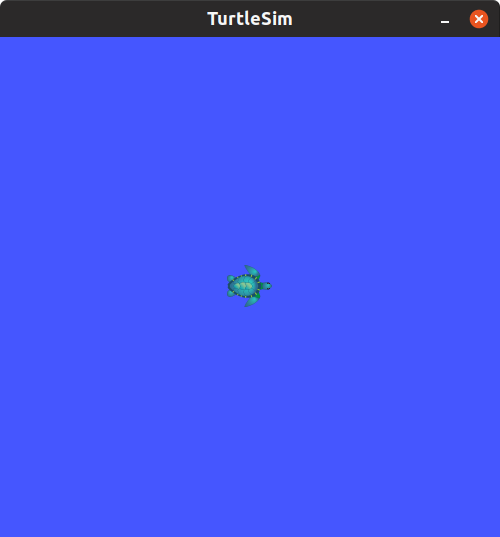
\includegraphics[width = 0.3\textwidth]{turtle_screenshot.png}
        \end{figure}
        \newpage
        Output from the third terminal:
        \begin{minted}[bgcolor=LightGray]{bash}
    Reading from keyboard
    ---------------------------
    Use arrow keys to move the turtle. 'q' to quit.          
        \end{minted}
        \item Keep the third terminal window and the turtlesim window open. With the third terminal
        window active, you should be able to control the turtle using the arrow keys. You should 
        see the turtle move and leave a trail behind it. Like this:

        \begin{figure}[H]
            \center
            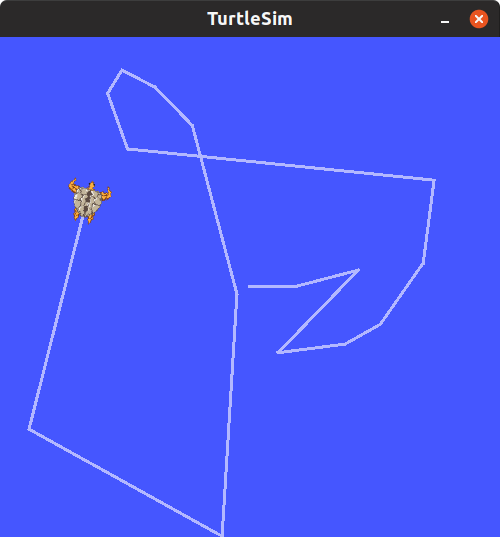
\includegraphics[width = 0.3\textwidth]{turtle_screenshot2.png}
        \end{figure}

        \item Let's now analyze what we did. First, we started a ROS master using the \texttt{roscore} 
        command. Next, we started two nodes, each using the \texttt{rosrun} command. The format for rosrun is:
        \begin{minted}[bgcolor=LightGray]{bash}
    :~$ rosrun <pkg> <type>
        \end{minted}
        \item There's nothing magical about rosrun. It is equivalent to going to the folder of turtlesim,
        finding the right executable, and running it directly, like a \texttt{./a.out} from C.
        \item To view the currently running nodes, in a new terminal, run:
        \begin{minted}[bgcolor=LightGray]{bash}
    :~$ rosnode list
        \end{minted}
        Output:
        \begin{minted}[bgcolor=LightGray]{bash}
    /rosout
    /teleop_turtle
    /turtlesim
        \end{minted}
        So we have three nodes: \texttt{/rosout}, which is like STDOUT but for ROS; \texttt{/turtlesim}, which is the turtle window;
         and \texttt{/teleop\_turtle}, which accepts the arrow key inputs.
        \item There must be some way by which \texttt{/teleop\_turtle} and \texttt{/turtlesim} are communicating.
        Let's investigate this. Run:
        \begin{minted}[bgcolor=LightGray]{bash}
    :~$ rosnode info /turtlesim
        \end{minted}
        \newpage
        Output (by the way, use the TAB key for autocomplete):
        \begin{minted}[bgcolor=LightGray]{bash}
    --------------------------------------------------------------------------------
    Node [/turtlesim]
    Publications: 
        * /rosout [rosgraph_msgs/Log]
        * /turtle1/color_sensor [turtlesim/Color]
        * /turtle1/pose [turtlesim/Pose]
    
    Subscriptions: 
        * /turtle1/cmd_vel [geometry_msgs/Twist]
    
    Services: 
        * /clear
        * /kill
        * /reset
        * /spawn
        * /turtle1/set_pen
        * /turtle1/teleport_absolute
        * /turtle1/teleport_relative
        * /turtlesim/get_loggers
        * /turtlesim/set_logger_level
    
    
    contacting node http://akb-G3-3579:36561/ ...
    Pid: 21017
    Connections:
        * topic: /rosout
        * to: /rosout
        * direction: outbound (54721 - 127.0.0.1:38478) [53]
        * transport: TCPROS
        * topic: /turtle1/cmd_vel
        * to: /teleop_turtle (http://akb-G3-3579:40119/)
        * direction: inbound (33248 - akb-G3-3579:53883) [56]
        * transport: TCPROS
    
        \end{minted}
        And run:
        \begin{minted}[bgcolor=LightGray]{bash}
    :~$ rosnode info /teleop_turtle
        \end{minted}
        Output:
        \begin{minted}[bgcolor=LightGray]{bash}
    --------------------------------------------------------------------------------
    Node [/teleop_turtle]
    Publications: 
        * /rosout [rosgraph_msgs/Log]
        * /turtle1/cmd_vel [geometry_msgs/Twist]
    
    Subscriptions: None
    
    Services: 
        * /teleop_turtle/get_loggers
        * /teleop_turtle/set_logger_level
    
    
    contacting node http://akb-G3-3579:40119/ ...
    Pid: 21190
    Connections:
        * topic: /rosout
        * to: /rosout
        * direction: outbound (53883 - 127.0.0.1:33246) [22]
        * transport: TCPROS
        * topic: /turtle1/cmd_vel
        * to: /turtlesim
        * direction: outbound (53883 - 127.0.0.1:33248) [20]
        * transport: TCPROS
        \end{minted}
        You can ignore most of the output. Pay attention to the topics being published
        and subscribed to. Specifically, observe that \texttt{/teleop\_turtle} publishes 
        to \texttt{/turtle1/cmd\_vel} while \texttt{/turtlesim} is subscribed to it. This could be 
        the mechanism by which the instructions are being communicated.

        \item Let's dig even deeper. Run:
        \begin{minted}[bgcolor=LightGray]{bash}
    :~$ rostopic list    
        \end{minted}
        Output:
        \begin{minted}[bgcolor=LightGray]{bash}
    /rosout
    /rosout_agg
    /turtle1/cmd_vel
    /turtle1/color_sensor
    /turtle1/pose
        \end{minted}
        Which is a list of the currently active topics. Now run (use TAB!):
        \begin{minted}[bgcolor=LightGray]{bash}
    :~$ rostopic echo /turtle1/cmd_vel
        \end{minted}
        Do this in a separate window, and observe what happens when you command the turtle using
        \texttt{/teleop\_turtle}. Output:
        \begin{minted}[bgcolor=LightGray]{bash}
    
    linear: 
    x: 2.0
    y: 0.0
    z: 0.0
    angular: 
    x: 0.0
    y: 0.0
    z: 0.0
    ---
    linear: 
    x: 0.0
    y: 0.0
    z: 0.0
    angular: 
    x: 0.0
    y: 0.0
    z: 2.0
    ---
    ...
        \end{minted}
        It would seem that this is indeed the way the commands are transmitted between the nodes.
        
        \item Another utility exists to observe the relation between multiple nodes. Try:
        \begin{minted}[bgcolor=LightGray]{bash}
    :~$ rqt_graph
        \end{minted}
        Initially, the graph is like this:
        \begin{figure}[H]
            \center
            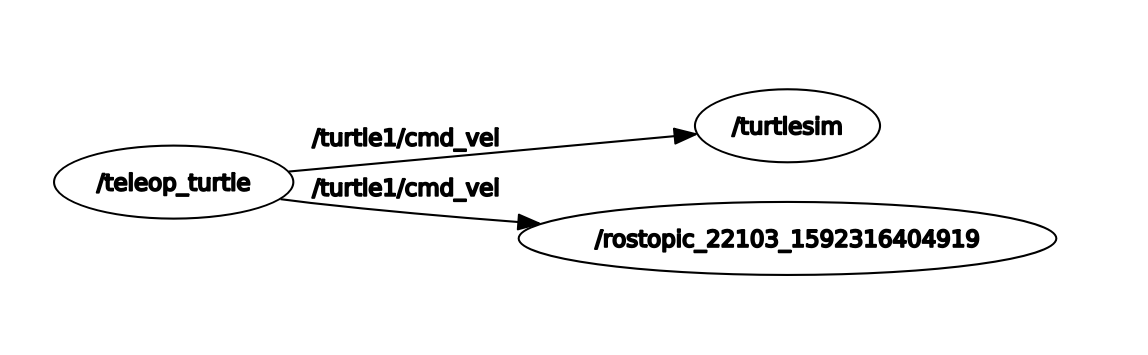
\includegraphics[width = 0.75\textwidth]{graph1.png}
        \end{figure}
        You can see the relation between \texttt{/teleop\_turtle} and \texttt{/turtlesim}.
        The other node is due to the \texttt{rostopic echo /turtle1/cmd\_vel} command.
        Now, uncheck all the 'hide' options, and choose "Nodes/Topics(all)". The graph looks like:
        \begin{figure}[H]
            \center
            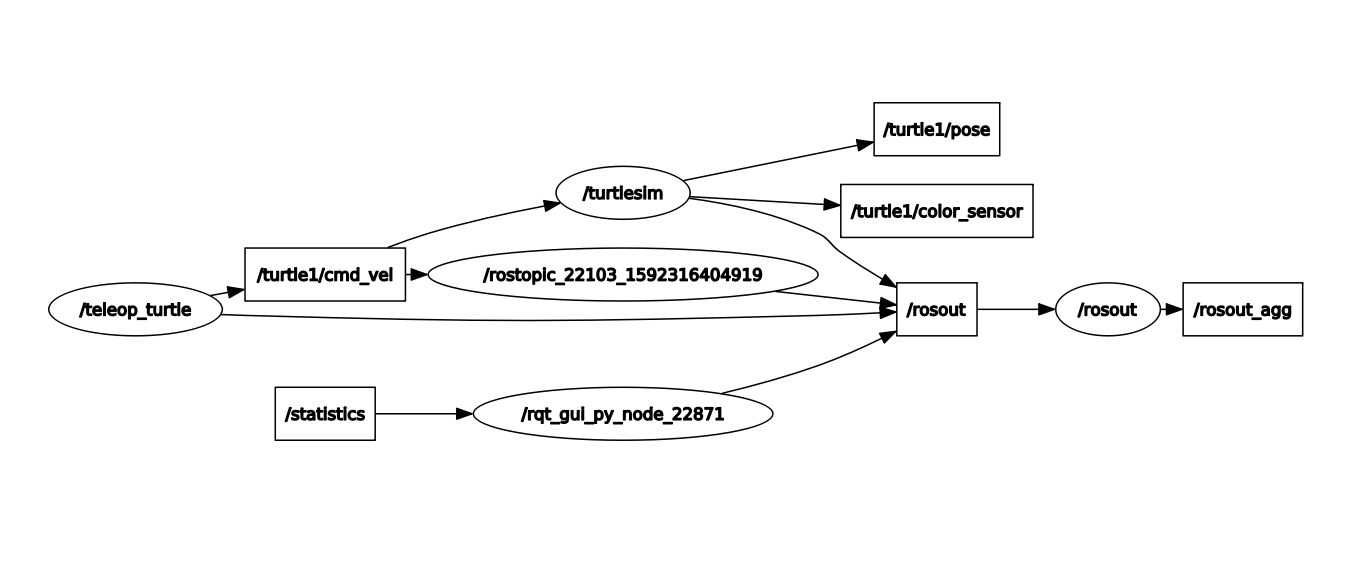
\includegraphics[width = 0.9\textwidth]{graph2.png}
        \end{figure}
        \texttt{rqt\_graph} is a valuable tool for visualizing and debugging.
        
        \item A key point: Publishers don't know who the subscribers are, and subscribers don't know who the 
        publishers are.

        \item Now, let's look at the message format used in \texttt{/turtle1/cmd\_vel}. Run:
        \begin{minted}[bgcolor=LightGray]{bash}
    :~$ rostopic type /turtle1/cmd_vel | rosmsg show
        \end{minted}
        The \texttt{|} operator takes the output of the preceding command and gives it as an argument 
        to the next command. Output:
        \begin{minted}[bgcolor=LightGray]{bash}
    geometry_msgs/Vector3 linear
    float64 x
    float64 y
    float64 z
    geometry_msgs/Vector3 angular
    float64 x
    float64 y
    float64 z
        \end{minted}
        This tells us that the message for \texttt{/turtle1/cmd\_vel} is composed of two \texttt{geometry\_msgs/Vector3},
        one of which is \texttt{linear} and the other \texttt{angular}. The \texttt{geometry\_msgs/Vector3} messages are themselves composed of
        three \texttt{float64}s -- \texttt{x}, \texttt{y} and \texttt{z}.
        \newpage
        \item It is possible to publish messages from the command line.
         With the three terminals from the beginning still running, open a fourth terminal and run:
        \begin{minted}[bgcolor=LightGray]{bash}
   :~$ rostopic pub -r 1 /turtle1/cmd_vel geometry_msgs/Twist '[2,0,0]' '[0,0,1]'
        \end{minted}
        And watch the turtle execute a circle.
        \item Let's break down that last command. \texttt{rostopic pub} -- we wish to publish; \texttt{-r 1} -- at a fixed rate of 1 Hz;
         \texttt{/turtle1/cmd\_vel} -- topic; \texttt{geometry\_msgs/Twist} -- message type; \texttt{'[2, 0, 0]' '[0, 0, 1]'} -- message contents.
        \item \texttt{/turtlesim} only uses \texttt{x} from \texttt{linear} and \texttt{z} from \texttt{angular}. It ignores the other two values.
        
        \item As a final demonstration, close all terminals, reopen five new terminals and run (one in each terminal):
        \begin{minted}[bgcolor=LightGray]{bash}
    :~$ roscore 
    :~$ rosrun turtlesim turtlesim_node __name:=A
    :~$ rosrun turtlesim turtlesim_node __name:=B
    :~$ rosrun turtlesim turtle_teleop_key __name:=C
    :~$ rosrun turtlesim turtle_teleop_key __name:=D
        \end{minted}
        What do you think will happen? Will \texttt{C} control \texttt{A} and \texttt{D}, \texttt{B}? Or vice-versa? Experiment and check.
        \item With the other terminals still open, run \texttt{rqt\_graph} and see the result.
        \begin{figure}[H]
            \center
            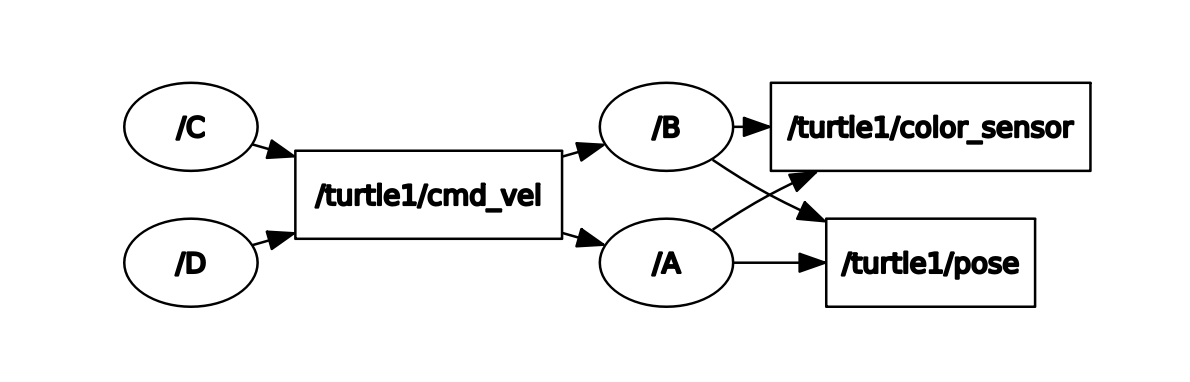
\includegraphics[width = 0.75\textwidth]{graph3.png}
        \end{figure}
        \item This should serve as an important lesson: Nodes are loosely coupled in nature. They are as independent as possible.
        \item Lastly, try the \texttt{roswtf} command.
        \item This section was adapted from \url{http://wiki.ros.org/ROS/Tutorials/UnderstandingNodes}, \url{http://wiki.ros.org/ROS/Tutorials/UnderstandingTopics}
        and \emph{A Gentle Introduction to ROS, Chapter Two}
    \end{enumerate}
    \section{Looking ahead}
    Next time, we will be creating our first ROS package and writing our first ROS nodes. 
\end{document}